\documentclass[12pt]{report}
\usepackage{graphicx}

\begin{document}


\title{Music App Usability Report}
\author{Jeff Fennell}
\date{September 2014}
\maketitle

The purpose of this study was to analyze two of the top music applications in existance to determine which has been more optimized for user interaction. Test subjects with different skill levels and domain knowledge of the platforms performed several tasks on both the iTunes and Spotify desktop applications. Based on the results, and using efficiency, learnability, and satisfaction as metrics for quantifying usability of the two systems, it has been decided that the Spotify platform is more usable.

The first task the test subjects performed was started on the main music library of the application. Users were asked to create a new playlist with the title "Hello World".  The second task testers were asked to perform was to make use of the automated radio, a feature that is present in both platforms. Users were asked to start the radio and create a station adapted to the artist "Tiesto". Again, the testers were timed to test efficiency of the system. The final task was to havigate to a pre-created playlist on the application, and turn on the playlist to loop indefinitely. For each of the tasks, the amount of time it took each user to complete the task was noted, as well as the number and nature of errors. Users were also asked questions to determine their level of satisfaction with each of the systems.

\section{Efficiency}

Spotify users proved to be more efficient in the first task of creating a playlist. The average time to create a playlist in Spotify was 11.17 seconds, while the average time to perform the same task in iTunes took an average of 16.34 seconds. 4 out of 7 users testing spotify actually completed the task faster than the quickest iTunes time recorded. 3 out of these 4 Spotify testers rated their own familiarity of Spotify as being less than 5 out of 10. This speaks to the learnability of Spotify as well, as users with little domain knowledge were able to quickly complete the task. The iTunes testers' times were slightly higher, with the highest time overall being by an iTunes user who rated their domain knowledge of iTunes as a 9 out of 10. It took this user 26 seconds to create a playlist, a full 7 seconds longer than the slowest time recorded by a Spotify tester. The slowest iTunes tester noted that iTunes frequently updates the user interface, therefore making it difficult to stay familiar with how to use certain features of the software.

Test subjects again proved to be much more efficient in performing the second task in Spotfy than in iTunes. The average time to complete the task in Spotify was 23.19 seconds. In iTunes, it generally took more than 7 seconds longer to complete the task, with the average time being 30.4 seconds.

\section{Errors}

In performing the first task, there were relatively few errors. Again, Spotify yielded better results, with users having only 2 errors out of the 7 tests. ITunes comparatively had 8 errors, for the 8 different tests. In Spotify, one erro

\section{Satisfaction}

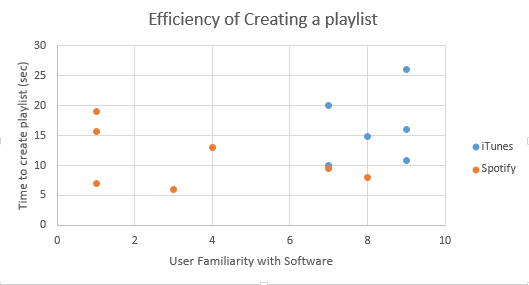
\includegraphics[width=\textwidth]{chart1.png}

\end{document}